\documentclass{article}

\usepackage{enumerate}
\usepackage{amssymb}
\usepackage{amsmath}
\usepackage{algorithm}
\usepackage{physics}
\usepackage{listings}
\usepackage[noend]{algpseudocode}
\usepackage{graphicx}

\graphicspath{ {./} }

\topmargin=-0.45in
\evensidemargin=0in
\oddsidemargin=0in
\textwidth=6.5in
\textheight=9.0in
\headsep=0.25in

\title{Chem 195: Problem Set 4}
\author{Michael Stephen Chen}


\begin{document}
\maketitle
\pagebreak

\section*{Problem 1}
\begin{enumerate}[i)]
  \item 
    \begin{align*}
      \matrixel{\phi_A}{x^4y^4}{\phi_B} &= \int_{-\infty}^{\infty} e^{-\alpha [(x-x_A)^2 - (y-y_A)^2]}x^4y^4e^{-\alpha [(x-x_B)^2 - (y-y_B)^2]} dx dy \\
      &= \int_{-\infty}^{\infty} e^{-(x-x_A)^2}x^4e^{-(x-x_B)^2} dx \int_{-\infty}^{\infty} e^{-(y-y_A)^2}y^4e^{-(y-y_B)^2} dy \\
      &= s(x_A,x_B)\left[\frac{3}{16\alpha^2} + \frac{3x_P^2}{2\alpha}+x_P^4\right]s(y_A,y_B)\left[\frac{3}{16\alpha^2} + \frac{3y_P^2}{2\alpha}+y_P^4\right] \\
      &= \frac{\pi}{2}\left[\frac{3}{16\alpha^2} + \frac{3x_P^2}{2\alpha}+x_P^4\right]\left[\frac{3}{16\alpha^2} + \frac{3y_P^2}{2\alpha}+y_P^4\right]e^{-\alpha [(x_A-x_B)^2 - (y_A-y_B)^2]/2}
    \end{align*}

  \item Variationally optimal $E_0$ estimates for various anharmonic factors with 225 basis functions:
    \begin{center}
      $\begin{array}{c|c}
        a & E_0 \\ \hline
        0.001 & 1.0006 \\ 
        0.010 & 1.0050 \\ 
        0.100 & 1.0329 \\ 
        1.000 & 1.1403 \\ 
        10.000 & 1.4151 \\ 
        100.000 & 1.9765 \\ 
      \end{array}$
    \end{center}

  \item Note that the wavefunction for the 2D harmonic oscillator is as follows:
    $$\psi_{0}(0) = \left( \frac{\alpha}{\pi} \right)^{\frac{1}{2}} e^{-\alpha(x^2 + y^2)/2}$$
    Thus the anharmonic perturbation is given by
    \begin{align*}
      \matrixel{\psi_0(0)}{x^4y^4}{\psi_0(0)} &= \left(\frac{\alpha}{\pi}\right)^{\frac{1}{2}} \int_{-\infty}^{\infty} e^{-\alpha x^2}x^4 dx \int_{-\infty}^{\infty} e^{-\alpha y^2}y^4 dy \\
      &= \frac{\alpha}{\pi} \left( \frac{3\sqrt{\pi}}{4\alpha^{5/2}} \right)^2 \\
      &= \frac{\alpha}{\pi} \frac{9\pi}{16\alpha^5} \\
      &= \frac{9}{16\alpha^4}
    \end{align*}
    
    The estimated gorund state energies using the perturbation method are as follows:
    \begin{center}
      $\begin{array}{c|c}
        a & E_0 \\ \hline
        0.001 & 1.0000 \\ 
        0.010 & 1.0004 \\ 
        0.100 & 1.0035 \\ 
        1.000 & 1.0352 \\ 
        10.000 & 1.3516 \\ 
        100.000 & 4.5156 \\
      \end{array}$
    \end{center}

    For small anharmonic factors $a$, the perturbation method appears to give similar results, as compared to part (ii). However for larger factors, the estimate varies greatly. So which estimate is more accurate? Given that our perturbation estimate only considers the linear anharmonic term, it should come as no surprise that the estimate will be poorer for larger values of $a$. To make the perturbation method more accurate, we would need to include more and more higher order terms. The estimate appears to be especially poor for $a=100$.

  \item Below is a plot depicting the variational estimate for the ground state energy as a function of the anharmonic term $a$.
    \begin{center}
      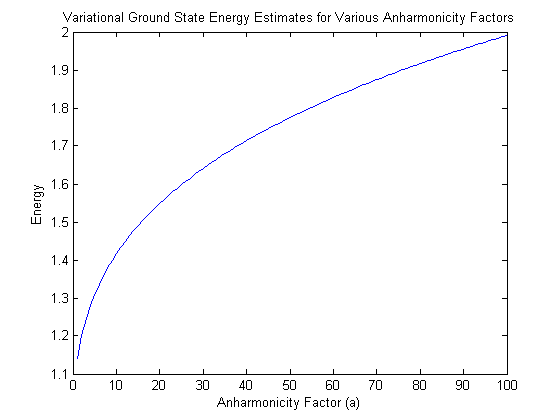
\includegraphics[scale=0.75]{prob1part4}
    \end{center}

  \item Below are the contour plots for the variationally estimated ground states for various anharmonic factors and with 225 basis functions.
    \begin{center}
      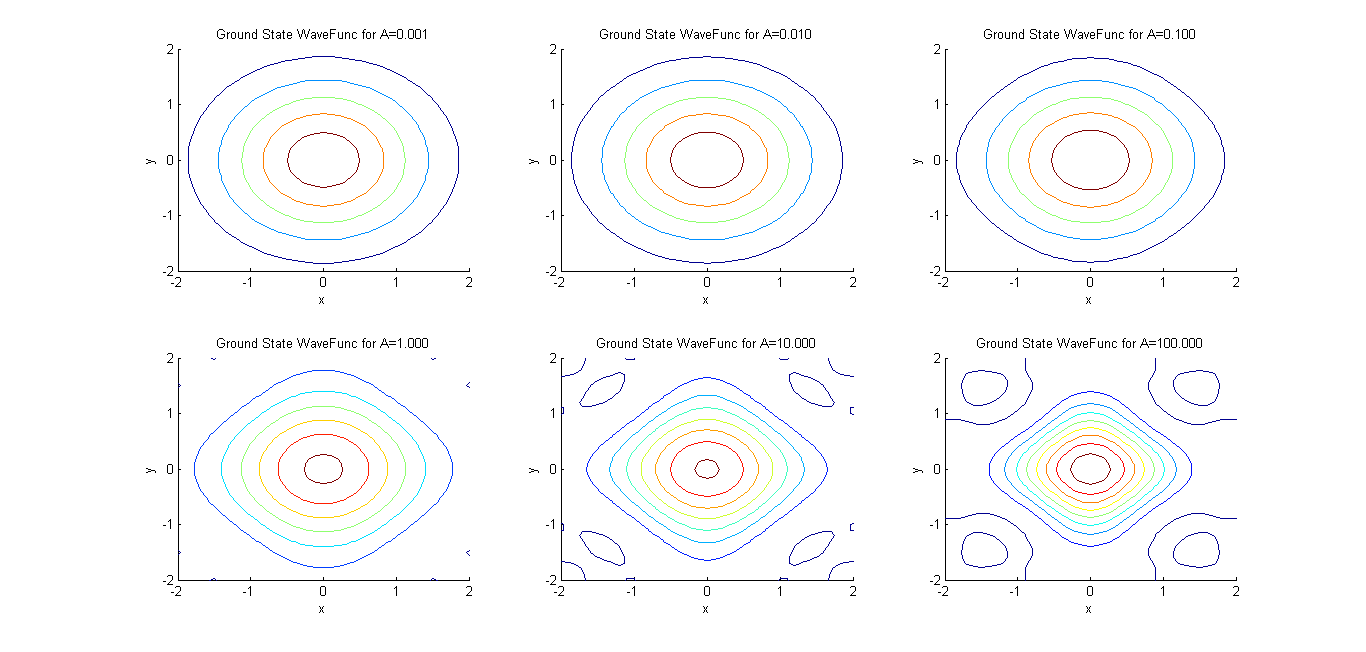
\includegraphics[scale=0.5]{prob1part5}
    \end{center}

      The anharmonic wavefunctions, take on a "diamond" shape with larger anharmonic factors. This is in contrast to the harmonic case that has spherical contour lines. To rationalize the anharmonic shape we can consider the anharmonic term as an addition to the potential. That's why along the axes, where the anharmonc term $x^4y^4 = 0$, the wave function contour lines "point outward" because there is no anharmonic gain to the energy. However moving away from the axes, the contour lines curve inward because of the anharmonic energy gain, which maxes out $45^{\circ}$ from any axes because that is where $x^4y^4$ is at a max.

    \item Refer to part (v) for the contour maps. It appears as though the shape of the wavefunction is noticeably changed by the time we reach $a = 0.1$. Beyond that, the nonlinear transformation of the wavefunction becomes more and more drastic. This is in lines with our previous assertion that the perturbation estimate becomes less accurate at larger $a$ because it cannot capture these nonlinear transformations, since the "Taylor-expansion-like" estimate only goes up to the linear term.

\end{enumerate}


\section*{Problem 2}
\begin{enumerate}[i)]
  \item We need to show that the wavefunction is an eigenfunction of the Hamiltonian operator
    \begin{align*}
      H\psi(x, y) &= \left[h(x) + h(y)\right] \left[ \frac{1}{\sqrt{2}} (\chi_1(x)\chi_2(y)) - \chi_2(x)\chi_1(y)\right] \\
      &= \frac{1}{\sqrt{2}} h(x) \left[ (\chi_1(x)\chi_2(y)) - \chi_2(x)\chi_1(y) \right] + \frac{1}{\sqrt{2}} h(y) \left[ (\chi_1(x)\chi_2(y)) - \chi_2(x)\chi_1(y) \right] \\
      &= \frac{1}{\sqrt{2}} [(E_1\chi_1(x))\chi_2(y)-(E_2\chi_2(x))\chi_1(y)] +  \frac{1}{\sqrt{2}} [\chi_1(x)(E_2\chi_2(y))-\chi_2(x)(E_1\chi_1(y))] \\
      &= \frac{1}{\sqrt{2}} [E_1\chi_2(y)\chi_1(x) + E_2\chi_1(x)\chi_2(y) - E_2\chi_2(x)\chi_1(y) - E_1\chi_2(x)\chi_1(y)] \\
      &= (E_1 + E_2) \left[ \frac{1}{\sqrt{2}} (\chi_1(x)\chi_2(y)) - \chi_2(x)\chi_1(y) \right] \\
      &= (E_1 + E_2) \psi(x, y)
    \end{align*}

    Thus we have shown that $\psi(x, y)$ is an eigenfunction of the Hamiltonian with an eigenvalue of $E_1 + E_2$ where $E_1$ is the eigenvalue for $\chi_1$ and $E_2$ is the eigenvalue for $\chi_2$.

  \item We can use our result from the previous problem to determine the energiess for the 2D antisym harmonic oscillator. The following equation gives the energy of the 2D HO as a function of the levels of the 1D HO wavefunctions $\chi_1$ and $\chi_2$. 
    \begin{align*}
      E &= E_1 + E_2 \\
      &= (n_1 + 1/2) + (n_2 + 1/2) \\
      &= n_1 + n_2 + 1
    \end{align*}

    Note that this result is identicle to the result from the previous problem set. However this time we impose the antisym constraint. From (2) we see this means that $\chi_1$ and $\chi_2$ must be distinct and that switching $\chi_1$ and $\chi_2$ does not result in a new distinct wavefuntion. The available energies are as follows.

    \begin{center}
      $\begin{array}{ccc|c}
       n & \chi_1 & \chi_2 & E \\ \hline
       1 &  1 & 0 & 2 \\ \hline
       2 &  2 & 0 & 3 \\ \hline
       3 & 2 & 1 & 4 \\
         & 3 & 0 & 4 \\ \hline
       4 & 3 & 1 & 5 \\
         & 4 & 0 & 5 \\ \hline
       5 & 5 & 0 & 6 \\
         & 4 & 1 & 6 \\
         & 3 & 2 & 6 \\ \hline
      \end{array}$
    \end{center}

    For even $n$, the number of degenerate states is $n/2$. For odd $n$, the number of degenerate states is $(n+1)/2$. 

  \item We need to show that the basis is antisymmetric or $\phi_A(x, y) = -\phi_A(y, x)$.
    \begin{align*}
      \phi_A(x,y) &= e^{-\alpha(x-x_A)^2 - \alpha(y-y_A)^2} - e^{-\alpha(x-y_A)^2 - \alpha(y-x_A)^2} \\
      \phi_A(y,x) &= e^{-\alpha(y-x_A)^2 - \alpha(x-y_A)^2} - e^{-\alpha(y-y_A)^2 - \alpha(x-x_A)^2} \\
      &= -(e^{-\alpha(x-x_A)^2 - \alpha(y-y_A)^2} - e^{-\alpha(x-y_A)^2 - \alpha(y-x_A)^2}) \\
      &= -\phi_A(x,y)
    \end{align*}

  \item 
    \begin{align*}
      S_{AB} &= \bra{\phi_A}\ket{\phi_B} \\
      &= \left( \bra{x_A,y_A}-\bra{y_A,x_A}\right)\left( \ket{x_B,y_B} - \ket{y_B,x_B}\right) \\
      &= \bra{x_A,y_A}\ket{x_B,y_B}-\bra{x_A,y_A}\ket{y_B,x_B}-\bra{y_A,x_A}\ket{x_B,y_B}+\bra{y_A,x_A}\ket{y_B,x_B} \\
      &= s(x_A,x_B)s(y_A,y_B) - s(x_A,y_B)s(y_A,x_B) - s(y_A,x_B)s(x_A,y_B) + s(y_A,y_B)s(x_A,x_B) \\
      &= 2s(x_A,x_B)s(y_A,y_B) - 2s(x_A,y_B)s(y_A,x_B)
    \end{align*}

  \item 
    \begin{align*}
      \matrixel{\phi_A}{h(x)}{\phi_B} &= \left( \bra{x_A,y_A}-\bra{y_A,x_A}\right)(h(x))\left( \ket{x_B,y_B} - \ket{y_B,x_B}\right) \\
      &= \matrixel{x_A,y_A}{h(x)}{x_B,y_B} - \matrixel{x_A,y_A}{h(x)}{y_B,x_B} - \matrixel{y_A,x_A}{h(x)}{x_B,y_B} + \matrixel{y_A,x_A}{h(x)}{y_B,x_B} \\
      &= \bra{y_A}\ket{y_B}\matrixel{x_A}{h(x)}{x_B} - \bra{y_A}\ket{x_B}\matrixel{x_A}{h(x)}{y_B} - \bra{x_A}\ket{y_B}\matrixel{y_A}{h(x)}{x_B} + \bra{x_A}\ket{x_B}\matrixel{y_A}{h(x)}{y_B} \\
      &= s(y_A,y_B)f(x_A,x_B) - s(y_A,x_B)f(x_A,y_B) - s(x_A,y_B)f(y_A,x_B) + s(x_A,x_B)f(y_A,y_B)\\
      \matrixel{\phi_A}{h(y)}{\phi_B} &= s(x_A,x_B)f(y_A,y_B) - s(x_A,y_B)f(y_A,x_B) - s(y_A,x_B)f(x_A,y_B) + s(y_A,y_B)f(x_A,x_B)\\
    \end{align*}

  \item 
    \begin{align*}
      \matrixel{\phi_A}{x^4y^4}{\phi_B} &= \left( \bra{x_A,y_A}-\bra{y_A,x_A}\right)(x^4y^4)\left( \ket{x_B,y_B} - \ket{y_B,x_B}\right) \\
      &= \matrixel{x_A,y_A}{x^4y^4}{x_B,y_B} - \matrixel{x_A,y_A}{x^4y^4}{y_B,x_B} - \matrixel{y_A,x_A}{x^4y^4}{x_B,y_B} + \matrixel{y_A,x_A}{x^4y^4}{y_B,x_B} \\
      &= \matrixel{y_A}{y^4}{y_B}\matrixel{x_A}{x^4}{x_B} - \matrixel{y_A}{y^4}{x_B}\matrixel{x_A}{x^4}{y_B} - \matrixel{x_A}{y^4}{y_B}\matrixel{y_A}{x^4}{x_B} + \matrixel{x_A}{y^4}{x_B}\matrixel{y_A}{x^4}{y_B} \\
      &= g(y_A,y_B)g(x_A,x_B) - g(y_A,x_B)g(x_A,y_B) - g(x_A,y_B)g(y_A,x_B) + g(x_A,x_B)g(y_A,y_B)\\
      &= 2g(x_A,x_B)g(y_A,y_B) - 2g(x_A,y_B)g(y_A,x_B)
    \end{align*}

  \item I expect the antisymmetric ground state to look like
    \begin{center}
    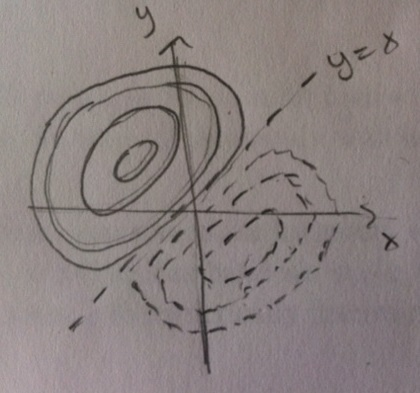
\includegraphics[scale=0.25]{prob2part7}
    \end{center}
    Where the solid contour lines are on opposite sides of the xy-plane with respect to the dotted contour lines. 
\end{enumerate}


\end{document}
